\documentclass{article}
\usepackage[utf8]{inputenc}
\usepackage[none]{hyphenat}
\usepackage[a4paper, total={7in, 9in}]{geometry}
\usepackage{fancyhdr}
\usepackage{parskip}
\usepackage{hyperref}
\usepackage{booktabs}
\usepackage{graphicx}

\title{Billboard Hot Songs Analysis with Spotify}
\author{Yuwei (Johnny) Meng}
\date{30 Apr 2024}

\begin{document}

\pagestyle{fancy}
\fancyhead[L]{JSC370}
\fancyhead[C]{Billboard Songs Analysis}
\fancyhead[R]{Johnny Meng}

\maketitle

\href{https://github.com/BullDF/billboard-songs-analysis-with-spotify/tree/main}{\textbf{Source Code on GitHub}}

\href{https://bulldf.github.io/billboard-songs-analysis-with-spotify/}{\textbf{Project Website}}

\section{Introduction}

Music, as a human culture, takes a large part in people's life for long. In the current era where technology thrives, countless digital musical softwares emerge, granting listeners with access to music at anytime, anywhere in the world. Concurrently emerged is the booming development of various music genres, each with its unique musical characteristics. Therefore, classifying music genres is an interesting research topic because, for one reason, a successful classification model can give insight into building a song recommendation system.

As an entry point to the project, a dataset on the ``Hot 100'' Billboard songs every week starting from 1958 is downloaded from Kaggle. The dataset contains 330087 rows and 7 columns that include information about the date of the song on Billboard, the name, the artist(s), and the rank on Billboard. In this project, only the name and the artist(s) columns are used.

Among the leading musical softwares, Spotify is a world-changing one. Founded in 2006 in Sweden, Spotify gradually attracted more and more users and built up a massive repository of worldwide music. Of this reason, a major portion of the data utilized in this data analysis project is obtained from Spotify through the Spotify web API and deemed credible and reliable. This portion of data contains the name of tracks, the artist(s), the track popularity, some audio features (see \hyperref[sec:appendixA]{appendix A} for full list) and in particular, a genre of music that the artist performs.

Given the genre, this project aims to use the aforementioned information extracted from Spotify to build and compare multiple machine learning models for the sake of classifying music genres. The models are mainly evaluated through classification accuracy scores and confusion matrices.

\section{Methodology}

The Billboard hot songs dataset from Kaggle is used as a reference. Starting with this list of 330087 tracks, to prevent overloading the Spotify API and keep the data at a manageable size, I randomly sampled 5000 tracks for the remaining analysis. Then I used the Spotify web API via the \texttt{Spotipy} Python library to access these songs on Spotify and extracted the audio features and popularity for these 5000 tracks. Given that some of these tracks are unavailable on Spotify, I obtained a dataset of 3823 tracks with their corresponding audio features. To obtain the labels, I selected 7 famous music genres (see \hyperref[sec:appendixB]{appendix B}). The Spotify API was then used to extract the music genre that the artists perform. If the music genre for an artist is not in the list, then it was marked as \textit{other}. For analysis, I merged the information into a single dataset with all the audio features and the genres of the tracks and split the dataset into a training set and a test set using an 80:20 ratio. All data wrangling steps were completed in R.

For the classification task, I constructed multiple machine learning models on the training set and evaluated them on the test set. These models included decision tree, random forest, gradient boosting, extreme gradient boosting (XGBoost), and neural network. The model construction and evaluation process was completed entirely in Python. The decision tree, random forest, and gradient boosting models were constructed using the \texttt{scikit-learn} package. For each type of models, I built one model using the default hyperparameters in \texttt{scikit-learn} and another using \(k\)-fold cross-validation to search over a reasonable set of hyperparameters. The XGBoost model was built using the \texttt{XGBoost} package, also with a careful search over a reasonable set of hyperparameters. The neural network featured 3 fully-connected layers and an output layer, implemented using the \texttt{PyTorch} framework. Batch normalization and dropout layers were included. The ReLU function was applied as activation throughout the model and the cross-entropy loss was used for the optimization task. Upon construction, all models were evaluated on the test dataset using accuracy score and confusion matrix.

\section{Exploratory Data Analysis}

Most exploratory data analysis steps have been completed in the previous part of this project (see EDA \href{https://github.com/BullDF/billboard-songs-analysis-with-spotify/blob/main/EDA/report.pdf}{report} and \href{https://bulldf.github.io/billboard-songs-analysis-with-spotify/EDA.html}{interactive visualizations}). Here I present some additional exploratory data analysis pertaining to the music genres for the following machine learning analysis.

\autoref{fig:music_genres} shows the 

\begin{figure}[htbp]
    \centering
    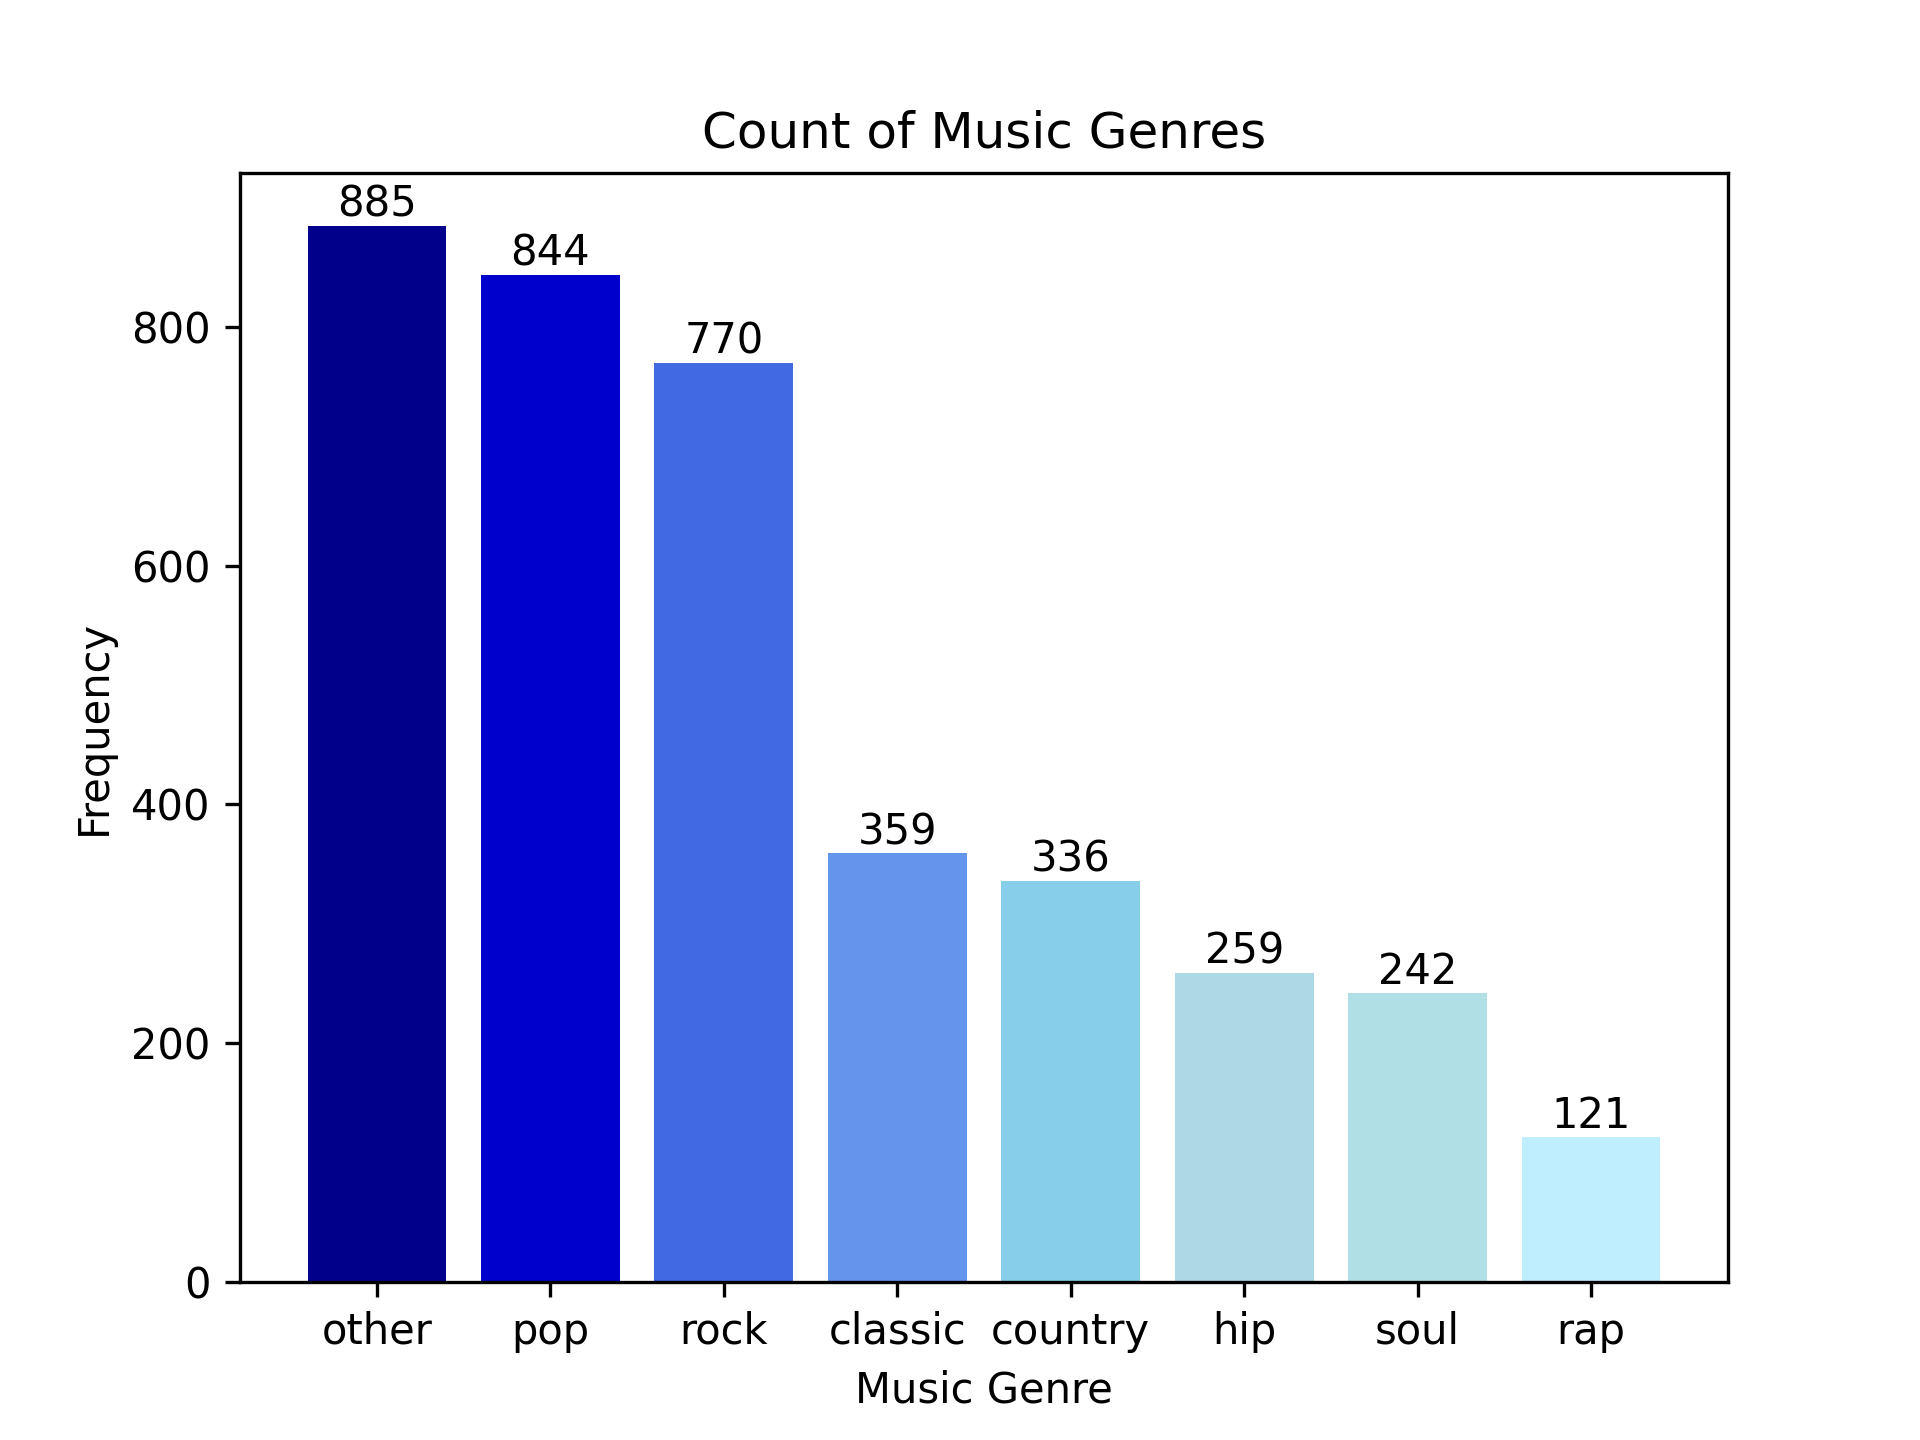
\includegraphics[width=10cm]{count_of_music_genres.png}
    \caption{Count of Music Genres}
    \label{fig:music_genres}
\end{figure}

\section{Results}

\autoref{tab:model_performance} shows the training accuracy and test accuracy for each machine learning model built in the analysis. As mentioned before, the decision tree, random forest, and gradient boosting models were constructed using the default hyperparameters as well as through \(k\)-fold cross-validation. 

\begin{table}[htbp]
    \centering
    \begin{tabular}{lcc}
        \toprule
        \textbf{Model} & \textbf{Training Accuracy} & \textbf{Test Accuracy} \\
        \midrule
        Decision Tree Default & 0.971 & 0.356 \\[3pt]
        Decision Tree CV & 0.487 & 0.440 \\[3pt]
        Random Forest Default & 0.971 & 0.505 \\[3pt]
        Random Forest CV & 0.804 & 0.473 \\[3pt]
        Gradient Boosting Default & 0.739 & 0.488 \\[3pt]
        Gradient Boosting CV & 0.81 & 0.79 \\[3pt]
        XGBoost & 0.93 & 0.89 \\[3pt]
        Neural Network & 0.551 & 0.486 \\
        \bottomrule
    \end{tabular}
    \caption{Model Performance}
    \label{tab:model_performance}
\end{table}

\section{Discussion}

\section{Conclusion}

\section{References}\label{sec:references}

\begin{itemize}
    \item \href{https://www.kaggle.com/datasets/dhruvildave/billboard-the-hot-100-songs}{Billboard ``The Hot 100'' Songs}
    \item \href{https://developer.spotify.com/documentation/web-api}{Spotify Web API Documentation}
    \item \href{https://spotipy.readthedocs.io/en/2.22.1/}{Spotipy Python Library Documentation}
    \item Python Package Documentations:
    \begin{itemize}
        \item \href{https://pytorch.org/docs/stable/torch.html}{\texttt{PyTorch}}
        \item \href{https://scikit-learn.org/stable/index.html}{\texttt{scikit-learn}}
        \item \href{https://xgboost.readthedocs.io/en/stable/python/python_intro.html}{\texttt{XGBoost}}
    \end{itemize}
\end{itemize}

\pagebreak

\section{Appendices}

\subsection*{Appendix A: Full List of Spotify Audio Features}\label{sec:appendixA}

\begin{table}[htbp]
    \centering
    \begin{tabular}{l p{0.7\textwidth}}
        \toprule
        \textbf{Audio Feature} & \textbf{Description} \\
        \midrule

        acousticness & A confidence measure from 0.0 to 1.0 of whether the track is acoustic. 1.0 represents high confidence the track is acoustic. \\[3pt]

        danceability & Danceability describes how suitable a track is for dancing based on a combination of musical elements including tempo, rhythm stability, beat strength, and overall regularity. A value of 0.0 is least danceable and 1.0 is most danceable. \\[3pt]

        duration\_ms & The duration of the track in milliseconds. \\[3pt]

        energy & Energy is a measure from 0.0 to 1.0 and represents a perceptual measure of intensity and activity. Typically, energetic tracks feel fast, loud, and noisy. For example, death metal has high energy, while a Bach prelude scores low on the scale. Perceptual features contributing to this attribute include dynamic range, perceived loudness, timbre, onset rate, and general entropy. \\[3pt]

        instrumentalness & Predicts whether a track contains no vocals. "Ooh" and "aah" sounds are treated as instrumental in this context. Rap or spoken word tracks are clearly "vocal". The closer the instrumentalness value is to 1.0, the greater likelihood the track contains no vocal content. Values above 0.5 are intended to represent instrumental tracks, but confidence is higher as the value approaches 1.0. \\[3pt]

        liveness & Detects the presence of an audience in the recording. Higher liveness values represent an increased probability that the track was performed live. A value above 0.8 provides strong likelihood that the track is live. \\[3pt]

        loudness & The overall loudness of a track in decibels (dB). Loudness values are averaged across the entire track and are useful for comparing relative loudness of tracks. Loudness is the quality of a sound that is the primary psychological correlate of physical strength (amplitude). Values typically range between -60 and 0 dB. \\[3pt]

        mode & Mode indicates the modality (major or minor) of a track, the type of scale from which its melodic content is derived. Major is represented by 1 and minor is 0. \\[3pt]

        speechiness & Speechiness detects the presence of spoken words in a track. The more exclusively speech-like the recording (e.g. talk show, audiobook, poetry), the closer to 1.0 the attribute value. Values above 0.66 describe tracks that are probably made entirely of spoken words. Values between 0.33 and 0.66 describe tracks that may contain both music and speech, either in sections or layered, including such cases as rap music. Values below 0.33 most likely represent music and other non-speech-like tracks. \\[3pt]

        valence & A measure from 0.0 to 1.0 describing the musical positiveness conveyed by a track. Tracks with high valence sound more positive (e.g. happy, cheerful, euphoric), while tracks with low valence sound more negative (e.g. sad, depressed, angry). \\
        \bottomrule
    \end{tabular}
\end{table}

\pagebreak

\subsection*{Appendix B: Selected Music Genres}\label{sec:appendixB}

\begin{table}[htbp]
    \centering
    \begin{tabular}{l}
        \toprule
        \textbf{Music Genre} \\
        \midrule
        rap \\[3pt]
        hip \\[3pt]
        classic \\[3pt]
        soul \\[3pt]
        country \\[3pt]
        pop \\[3pt]
        rock \\[3pt]
        other \\
        \bottomrule
    \end{tabular}
    \caption{Music Genres}
\end{table}



\end{document}